\section{Metoder til afl�sning af ADNS sensor}\label{sec:bilag_adnsaflaesning}
Under udabejdelsen af programkoden til at hente data fra sensoren, blev forskellige l�sninger overvejet. Disse l�sninger er kort gennemg�et herunder.

\subsection{L�sning 1}
Denne l�sning blev valgt, og er beskrevet i detaljer i sektion \ref{sec:aflaesning_af_sensor}, hvorfor den ikke gennemg�s her.

\subsection{L�sning 2}
Denne l�sning er bygget op omkring at hele sensorafl�sningen sker i et timerinterupt. N�r timerinteruptet sker starter afl�sningen af sensoren, hvorefter hastighedsreguleringen startes. Fordelen ved denne er at den er forholdsvis simpel at implementere, og intervallet mellem afl�sning af sensoren vil v�re forholdsvis konstant. Problemet med denne model er, at denne model bruger rigtigt meget tid p� at vente p� svar fra sensoren, som ikke kan bruges til noget andet.

\begin{figure}[htb]
  \centering
  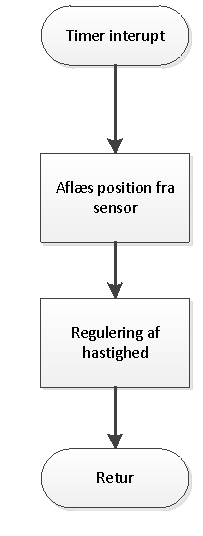
\includegraphics[scale=1]{ADNS_handling_met2.pdf}  
  \caption{Afl�sningsmetode 2}
  \label{fig:ADNS_handling_met2}
\end{figure}

\subsection{L�sning 3}
I denne l�sning afl�ses kun de to relevate data fra sensoren. Under start at microcontrolleren sendes foresp�rgsel om lav bytes en delta y v�rdien. N�r denne modtages, gemmes den, og der sendes foresp�rgsel om h�j byten af delta y. N�r delta y h�j modtages, gemmes denne og hastighedsreguleringen g�r i gang. Efter dette sendes foresp�rgsel om lav byte, og det hele starter forfra. Fordelen ved denne metode, er at der kun hentes data der skal benyttes. Detta kan ogs� se som v�rende en ulempe, da der derfor kun er disse til r�dighed ved fejlfindeing. Et problem med denne metode er at det ikke er muligt at verificere at det modtagede data er korrekt.

\begin{figure}[htb]
  \centering
  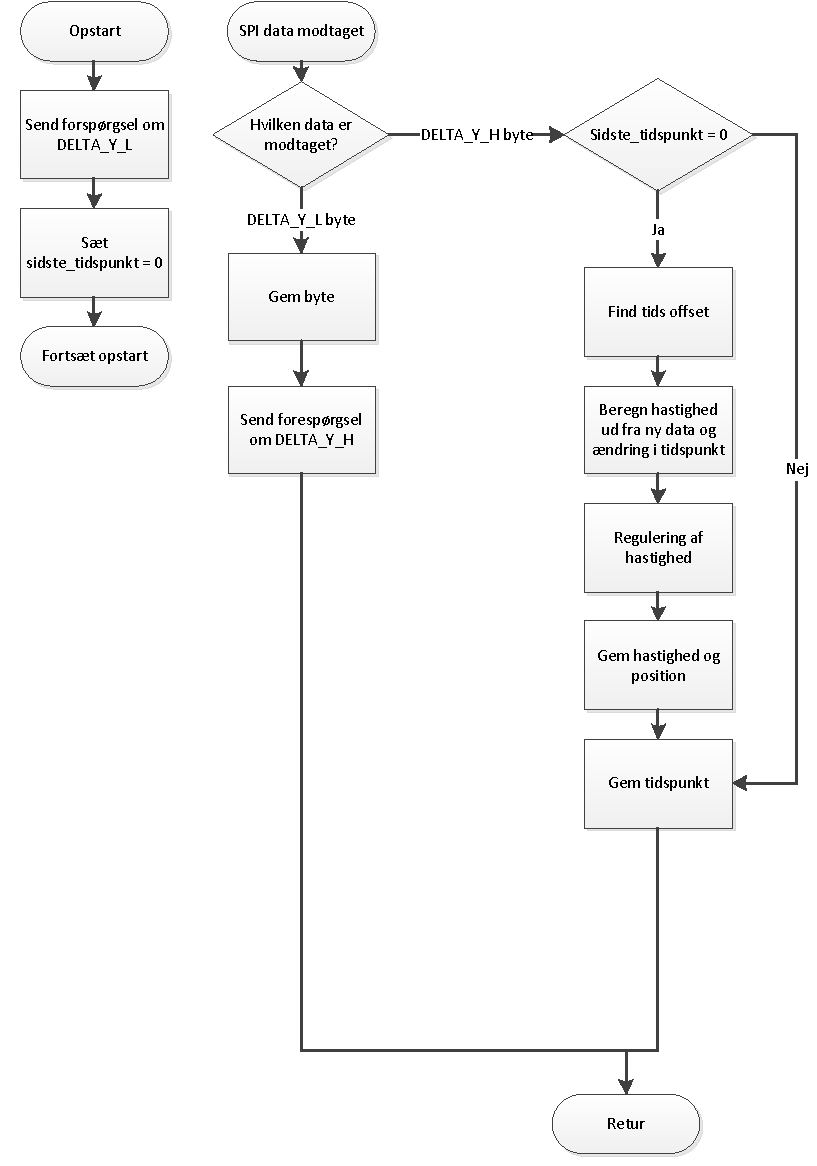
\includegraphics[scale=0.8]{ADNS_handling_met3.pdf}  
  \caption{Afl�sningsmetode 3}
  \label{fig:ADNS_handling_met3}
\end{figure}


\subsection{Begrundelse for valg}
%Umiddelbart er det i dette projekt kun relevant at 
%Det blev valgt at benytte l�sning 1, da der er en lang r�kke .... 

Til afhentning af data er l�sning 1 benyttet. Valget er truffet p� baggrund af, at denne model har en masse ekstra information fra sensoren. Dette ekstra info kan benyttes til at kontrollere, om sensoren rent faktisk er i en funktionel tilstand, og udfra dette kan der eventuelt senere opbygges programkode, der s�rger for at genstarte sensoren ved fejl under k�rslen. Ved at f.eks at have valgt l�sning to eller tre, ville en fejl i kommunikationen ikke opdages, og herved vil der ikke kunne tages h�jde for dette. Ved l�sning et er der mulighed for at kontrollere MOTION\footnote{V�rdi der viser sensorens tilstand}-og SQUAL\footnote{Surface Quality}-v�rdien fra sensoren, da disse giver et repr�sentativt billede af kvaliteten af de m�lte data og sensorens tilstand.